\subsection{相伴分次模同态的提升}

定理 1. 设 X、Y 为两个滤过群，其滤过 \((\mathbf{X}_n)\)、\((\mathbf{Y}_n)\) 由正规子群组成；设 \(u: \mathbf{X} \to \mathbf{Y}\) 为与滤过相容的同态。

\begin{enumerate}
\def\labelenumi{(\roman{enumi})}
\item
	假设滤过 \((\mathbf{X}_n)\) 是穷竭的。\(\operatorname{gr}(u)\) 为单射的充要条件是 \(u^{-1}(\mathbf{Y}_n) = \mathbf{X}_n\) 对所有 \(n \in \mathbf{Z}\) 成立。
\item
	假设下列条件之一成立：(α) X 完备且 Y Hausdorff；(β) Y 离散。则 gr(u) 为满射的充要条件是 \(Y_{n} = u(X_{n})\) 对所有 \(n \in Z\) 成立。
\end{enumerate}

\begin{enumerate}
\def\labelenumi{(\roman{enumi})}
\tightlist
\item
  说映射 \(\mathbf{gr}_n(u)\) 是单射，就是说

\[
\mathbf {X} _ {n} \cap^ {- 1} u ^ {1} (\mathbf {Y} _ {n + 1}) \subset \mathbf {X} _ {n + 1}.
\]

若 \(\bar{u}^1 (\mathbf{Y}_{n + 1}) = \mathbf{X}_{n + 1}\)，显然成立。反之，若

\[
\mathbf {X} _ {n} \cap^ {- 1} u (\mathbf {Y} _ {n + 1}) \subset \mathbf {X} _ {n + 1}
\]

	对所有 \(n\)，通过归纳 \(k\) 可得 \(\mathbf{X}_{n-k} \cap \bar{u}^1(\mathbf{Y}_{n+1}) \subset \mathbf{X}_{n+1}\) 对所有 \(n \in \mathbf{Z}\) 及所有 \(k \geqslant 0\) 成立。由于滤过 \((\mathbf{X}_n)\) 穷竭，可见对所有 \(n\)，\(\mathbf{X}\) 是各 \(\mathbf{X}_{n-k} (k \geqslant 0)\) 的并，因此 \(\bar{u}^1(\mathbf{Y}_{n+1}) \subset \mathbf{X}_{n+1}\) 对所有 \(n\) 成立，从而 \(\mathbf{X}_{n+1} \subset \bar{u}^1(\mathbf{Y}_{n+1})\)，证明完毕。

\item
  说映射 \(\mathrm{gr}_n(u)\) 是满射，就是说
\end{enumerate}

\[
\mathbf {Y} _ {n} = u (\mathbf {X} _ {n}) \mathbf {Y} _ {n + 1}.
\]

	若 \(Y_{n}=u(X_{n})\)，显然成立。反之，设 \(Y_{n}=u(X_{n})Y_{n+1}\) 对所有 \(n\in Z\) 成立。令 n 为整数，y 为 \(Y_{n}\) 中的元素；我们定义元素序列 \((x_{k})_{k\geq0}\)，其元素属于 \(X_{n}\)，使 \(x_{k}\in X_{n}\)、\(x_{k+1}\equiv x_{k} \pmod{X_{n+k}}\) 且 \(u(x_{k})\equiv y \pmod{Y_{n+k}}\) 对所有 \(k\geq0\) 成立。取 \(x_{0}\) 为 X 的单位元，这当然给出 \(u(x_{0})\equiv y \pmod{Y_{n}}\)。假设已构造 \(x_{k}\in X_{n}\)，使得 \(u(x_{k})\equiv y \pmod{Y_{n+k}}\)；则 \((u(x_{k}))^{-1}y\in Y_{n+k}\)；根据假设，存在 \(t\in X_{n+k}\)，使得 \(u(t)\equiv(u(x_{k}))^{-1}y \pmod{Y_{n+k+1}}\)，从而 \(u(x_{k}t)\equiv y \pmod{Y_{n+k+1}}\)；归纳构造只需取 \(x_{k+1}=x_{k}t\)。为此，若 Y 离散，则存在 \(k\geq0\) 使得 \(Y_{n+k}=\{e'\}\)（Y 的单位元），从而 \(u(x_{k})=y\)，因此在这种情形下已经证明对所有 n 有 \(u(X_{n})=Y_{n}\)。~现在假设 X 完备而 Y 是 Hausdorff 的。由于 \(x_{h}^{-1}x_{k}\in X_{n+k}\) 对 \(h\geq k\geq0\)，\((x_{k})\) 是 \(X_{n}\) 中的 Cauchy 序列；由于

\(X_{n}\) 是 X 中的闭集，因而完备，所以该序列在 \(X_{n}\) 中至少有一个极限 x。由 u 的连续性，\(u(x)\) 是序列 \((u(x_{k}))\) 在 Y 中的唯一极限，因为 Y 是 Hausdorff 的。但关系 \(u(x_{k}) \equiv y \pmod{Y_{n+k+1}}\) 表明 y 也是该序列的极限，从而 \(u(x) = y\)，这也证明了 \(u(X_{n}) = Y_{n}\)。

推论 1. 假设 X 是 Hausdorff 的且其滤过穷竭。则若 gr(u) 是单射，u 也是单射。

令 \(e, e'\) 分别为 X 和 Y 的单位元。于是

\[
\bar {u} ^ {1} (e ^ {\prime}) \subset \bigcap_ {n} \bar {u} ^ {1} (\mathbf {Y} _ {n}) = \bigcap_ {n} \mathbf {X} _ {n} = \{e \}
\]

由假设，推论得证。

推论 2. 假设下列条件之一成立：

(α) X 完备，Y 是 Hausdorff 的且其滤过穷竭；

(β) Y 离散且其滤过穷竭。

则若 \(\operatorname{gr}(u)\) 是满射，\(u\) 也是满射。

	在此情形下，\(\mathbf{Y} = \bigcup_{n}\mathbf{Y}_{n} = \bigcup_{n}u(\mathbf{X}_{n})\subset u(\mathbf{X}).\)

推论 3. 假设 X 和 Y 都是 Hausdorff 的，X 和 Y 的滤过穷竭，且 X 完备。则若 gr(u) 是双射，u 也是双射。

设 A 为局部环，m 为其极大理想，M 为 A-模；给 A 和 M 赋予 m-进滤过，并令 gr(A) 和 gr(M) 分别为与 A 和 M 相伴的分次环及分次 gr(A)-模。我们已经看到（第 3 节，例 3），典范映射 (11) 总是满射；现在考虑 M 的下列性质：

(GR) 典范映射

\[
\gamma_ {\mathbf {M}} \colon \operatorname{gr} (\mathbf {A}) \otimes_ {\mathbf {g r} _ {0} (\mathbf {A})} \operatorname{gr} _ {0} (\mathbf {M}) \rightarrow \operatorname{gr} (\mathbf {M})
\]

是双射。

命题 9. 设 A 为局部环，m 为其极大理想，M、N 为两个 A-模，u: N → M 为 A-同态。给 M 和 N 赋予 m-进滤过，并假设：(1) M 满足性质 (GR)；(2) gr₀(u): gr₀(N) → gr₀(M) 是单射。则 gr(u): gr(N) → gr(M) 是单射，N 和 P = Coker(u) 满足性质 (GR)，且对每个整数 n \textgreater{} 0 有 mⁿN = -¹u(mⁿM)。

立即验证可知，下图

\[
\begin{array}{c} \operatorname{gr} (\mathrm{A}) \otimes_ {\mathbf {g r} _ {0} (\mathrm{A})} \operatorname{gr} _ {0} (\mathrm{N}) \xrightarrow {1 \otimes \operatorname{gr} _ {0} (u)} \operatorname{gr} (\mathrm{A}) \otimes_ {\mathbf {g r} _ {0} (\mathrm{A})} \operatorname{gr} _ {0} (\mathrm{M}) \\ \gamma_ {\mathrm{N}} \Biggl \downarrow \\ \operatorname{gr} (\mathrm{N}) \xrightarrow [ \operatorname{gr} (u) ]{} \operatorname{gr} (\mathrm{M}) \end{array}
\]

是交换的。由于 \(\mathrm{gr}_{0}(\mathbf{A}) = \mathbf{A}/\mathfrak{m}\) 是域，假设蕴含 \(1 \otimes \mathrm{gr}_{0}(u)\) 是单射；又由于按假设 \(\gamma_{M}\) 是单射，\(\gamma_{M} \circ (1 \otimes \mathrm{gr}_{0}(u))\) 也是单射。这首先蕴含 \(\gamma_{N}\) 是单射，因而是双射，从而 \(\mathrm{gr}(u)\) 是单射。公式 \(\overline{u}^{1}(\mathfrak{m}^{n}\mathbf{M}) = \mathfrak{m}^{n}\mathbf{N}\) 随即由定理 1 (i) 得出。

此外，记 \(N' = u(N)\)，令 \(j: N' \to M\) 为典范嵌入。若 \(p: M \to P = M/N'\) 是典范同态，则在交换图

\pandocbounded{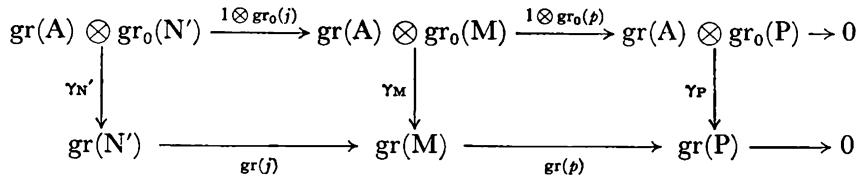
\includegraphics[keepaspectratio]{images/part002_c4775371.jpg}}

	下行是正合的（第 4 节，命题 2），而由第 4 节的命题 2 及 \(\mathrm{gr}_0(\mathbf{A})\) 是域这一事实，上行也正合。此外，\(\mathrm{gr}(j)\) 是单射（第 4 节，命题 2），因而 \(\mathrm{gr}_0(j)\) 是单射。对 \(j\) 应用论证的第一部分可知 \(\gamma_{\mathbf{N}'}\) 是双射；由于按假设 \(\gamma_{\mathbf{M}}\) 也是双射，故 \(\gamma_{\mathbf{P}}\) 是双射（第 I 章，§ 1，第 4 节，命题 2 的推论 2）。

推论。在命题 9 的假设下，若还假定 N 在 m-进滤过下是 Hausdorff 的，则 u 是单射。

这是因为 \(\operatorname{gr}(u)\) 是单射（定理 1 的推论 1）。

* 注。假设命题 9 的条件成立，并且下列条件之一也成立：

\begin{enumerate}
\def\labelenumi{(\arabic{enumi})}
\item
  m 是幂零的；
\item
  A 是 Noether 环且 P 是理想 Hausdorff 的（参见~§ 5，第 1 节）；
\end{enumerate}

则 P 是平坦 A-模。这由 \(\gamma_{P}\) 是双射及 § 5，第 2 节，定理 1 (iv) 得出，因为 A/m 是域。 *

